%*******10********20********30********40********50********60********70********80
\clearpage

\subsection{Result And Discussion}

In this section, the relationship between concrete's behavior of expansion and its losses on mechanical properties are discussed.

By RBSM, all information of the 3-dimensional cracking behavior can be recorded and analysis numerically. While it is with difficulties to summarized the behavior of expansion by the naked eye, all stress distribution and crack generation process are able to be analyzed numerically.

For example, in Figure \ref{fig:Total_Number_of_Cracks}, the relationship of total cracked interfaces and its relationship with residual compressive strength (in a ratio of the compressive strength of undamaged model) is presented.

It can be seen that as the total cracking interfaces number increase, the residual compressive strength decrease in all kinds of expansion applied.

\begin{figure}[ht]
\centering
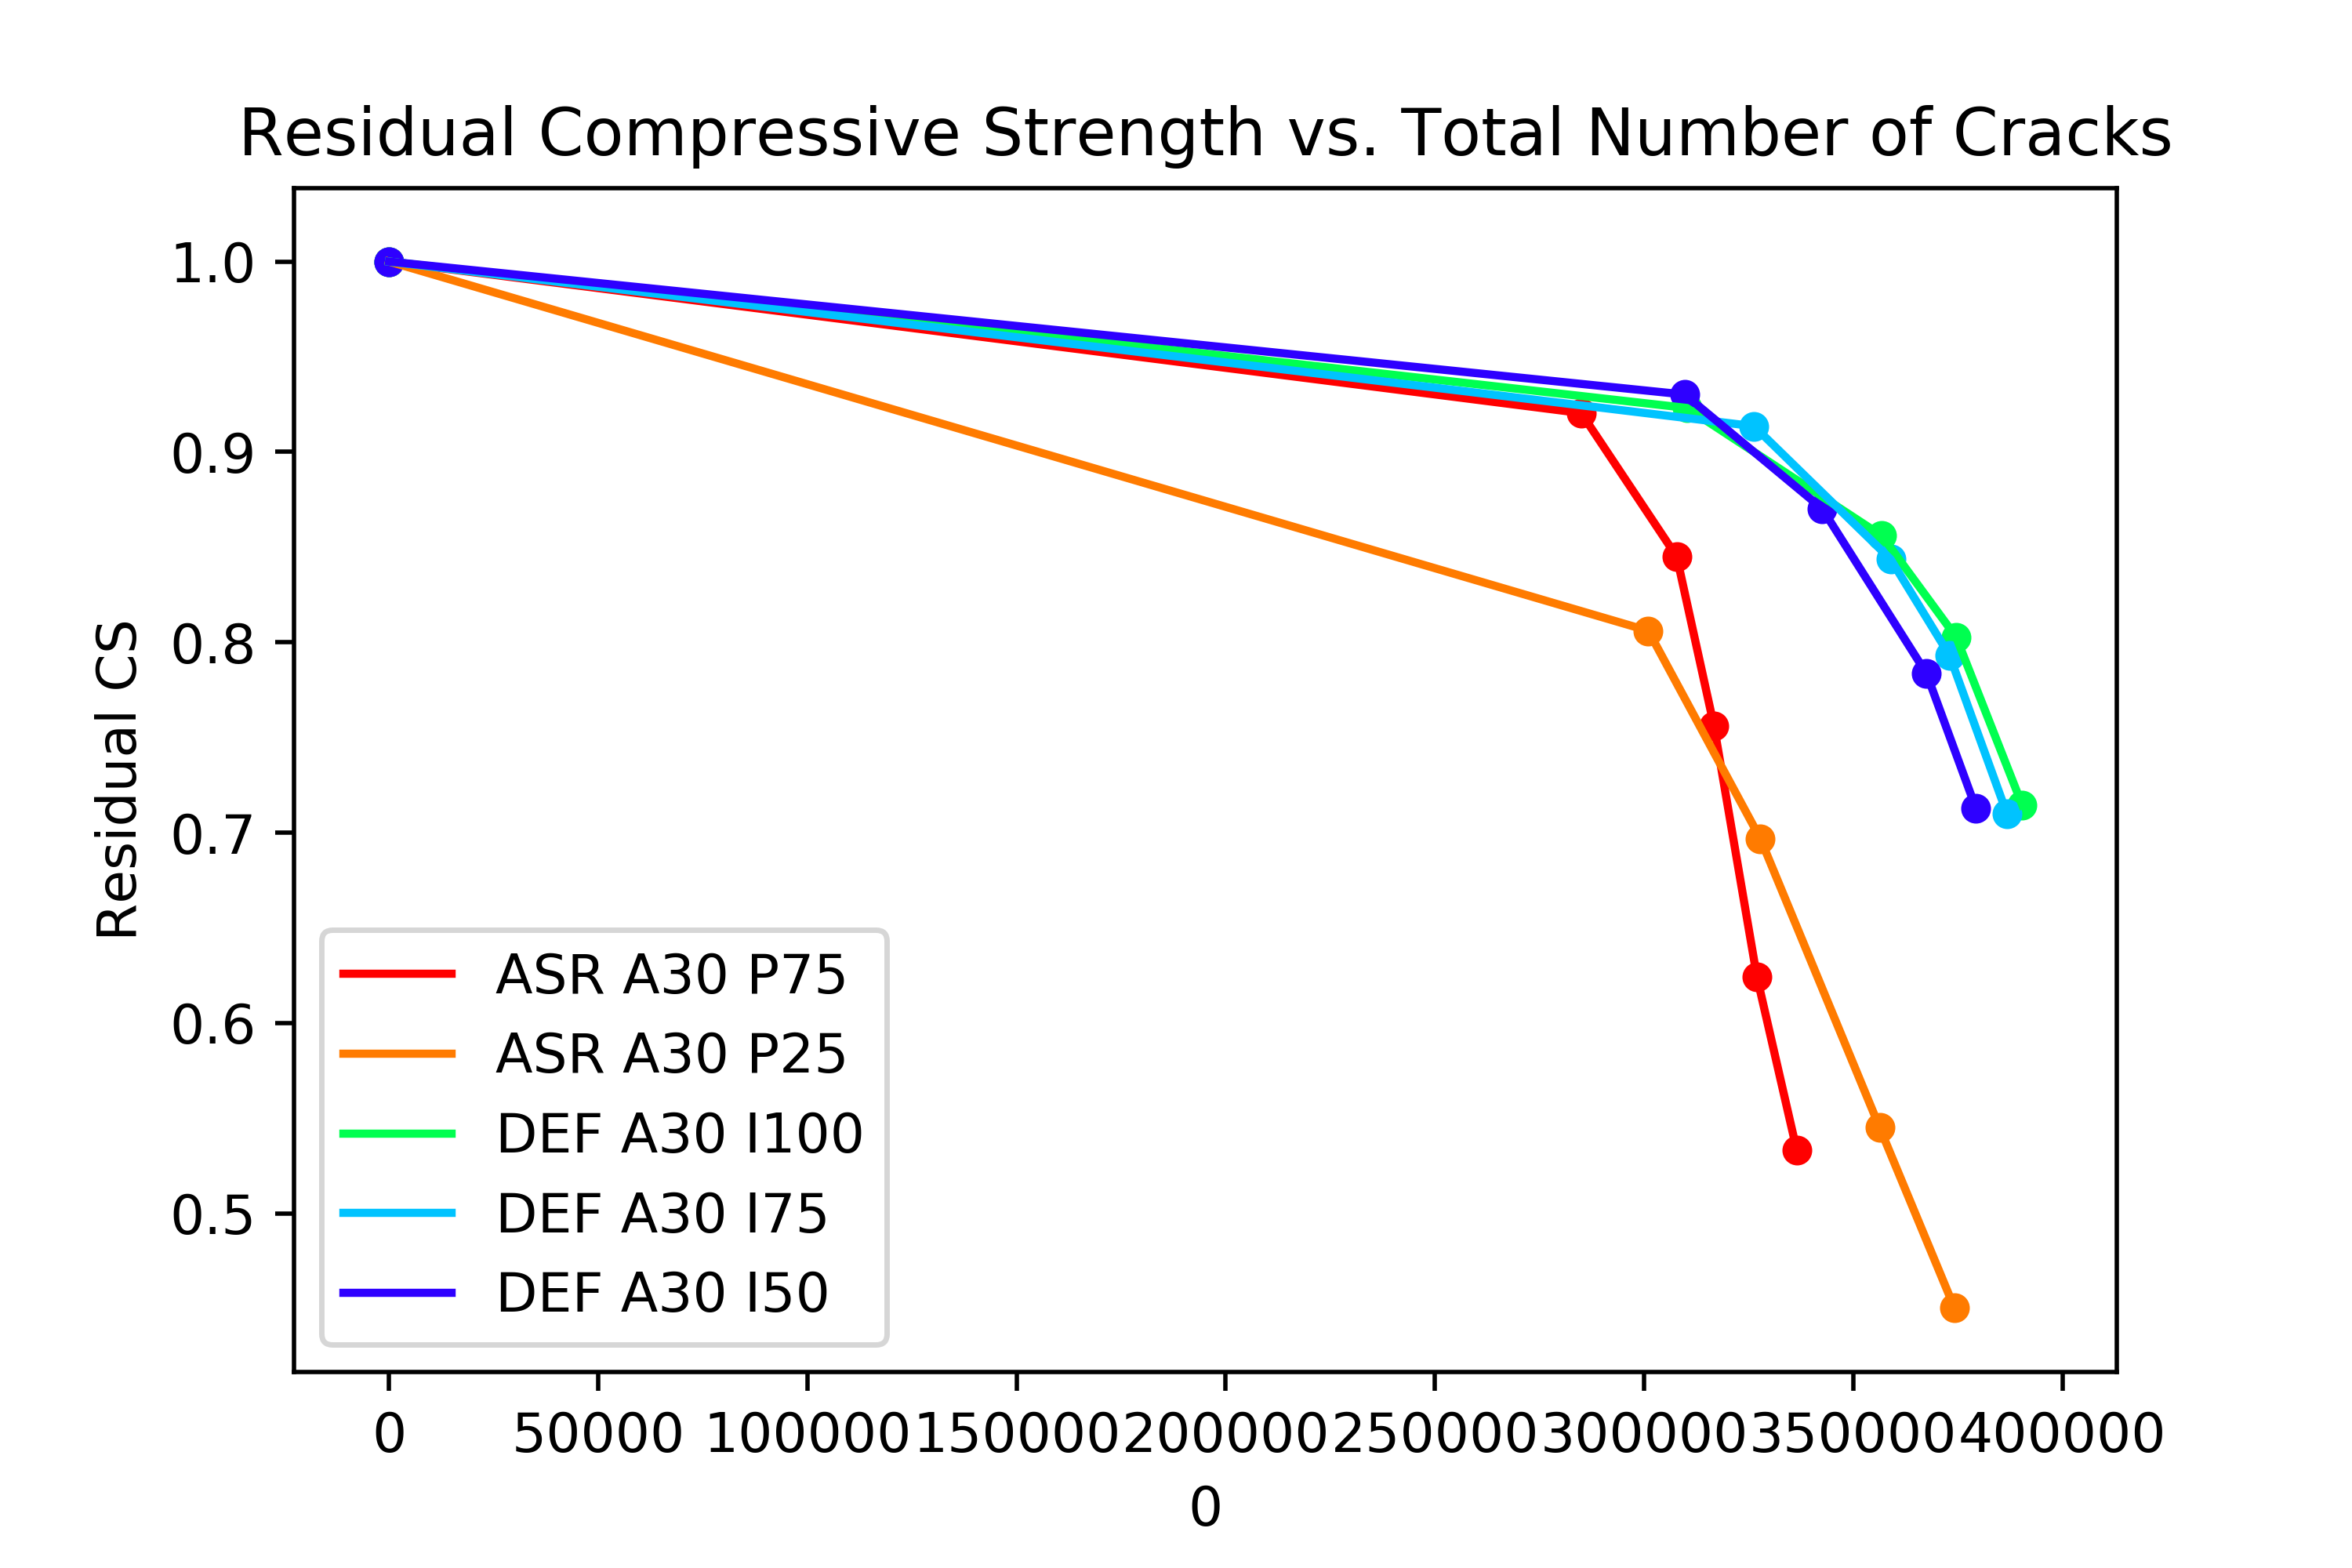
\includegraphics[width=.8\linewidth]{Files/exp_3D/Residual_Compressive_Strength_vs_Total_Number_of_Cracks.png}
  \caption{Residual Compressive Strength vs. Total Number of Cracks}
  \label{fig:Total_Number_of_Cracks}
\end{figure}

While structually, larger crack in width do represent larger damage, especially in its mechanical properties, here in Figure \ref{fig:Total_Number_of_Cracks_0.0005+} the relationship between total number of cracked interfaces larger than 0.0005mm and the residual compressive strength is plotted.

\begin{figure}[ht]
\centering
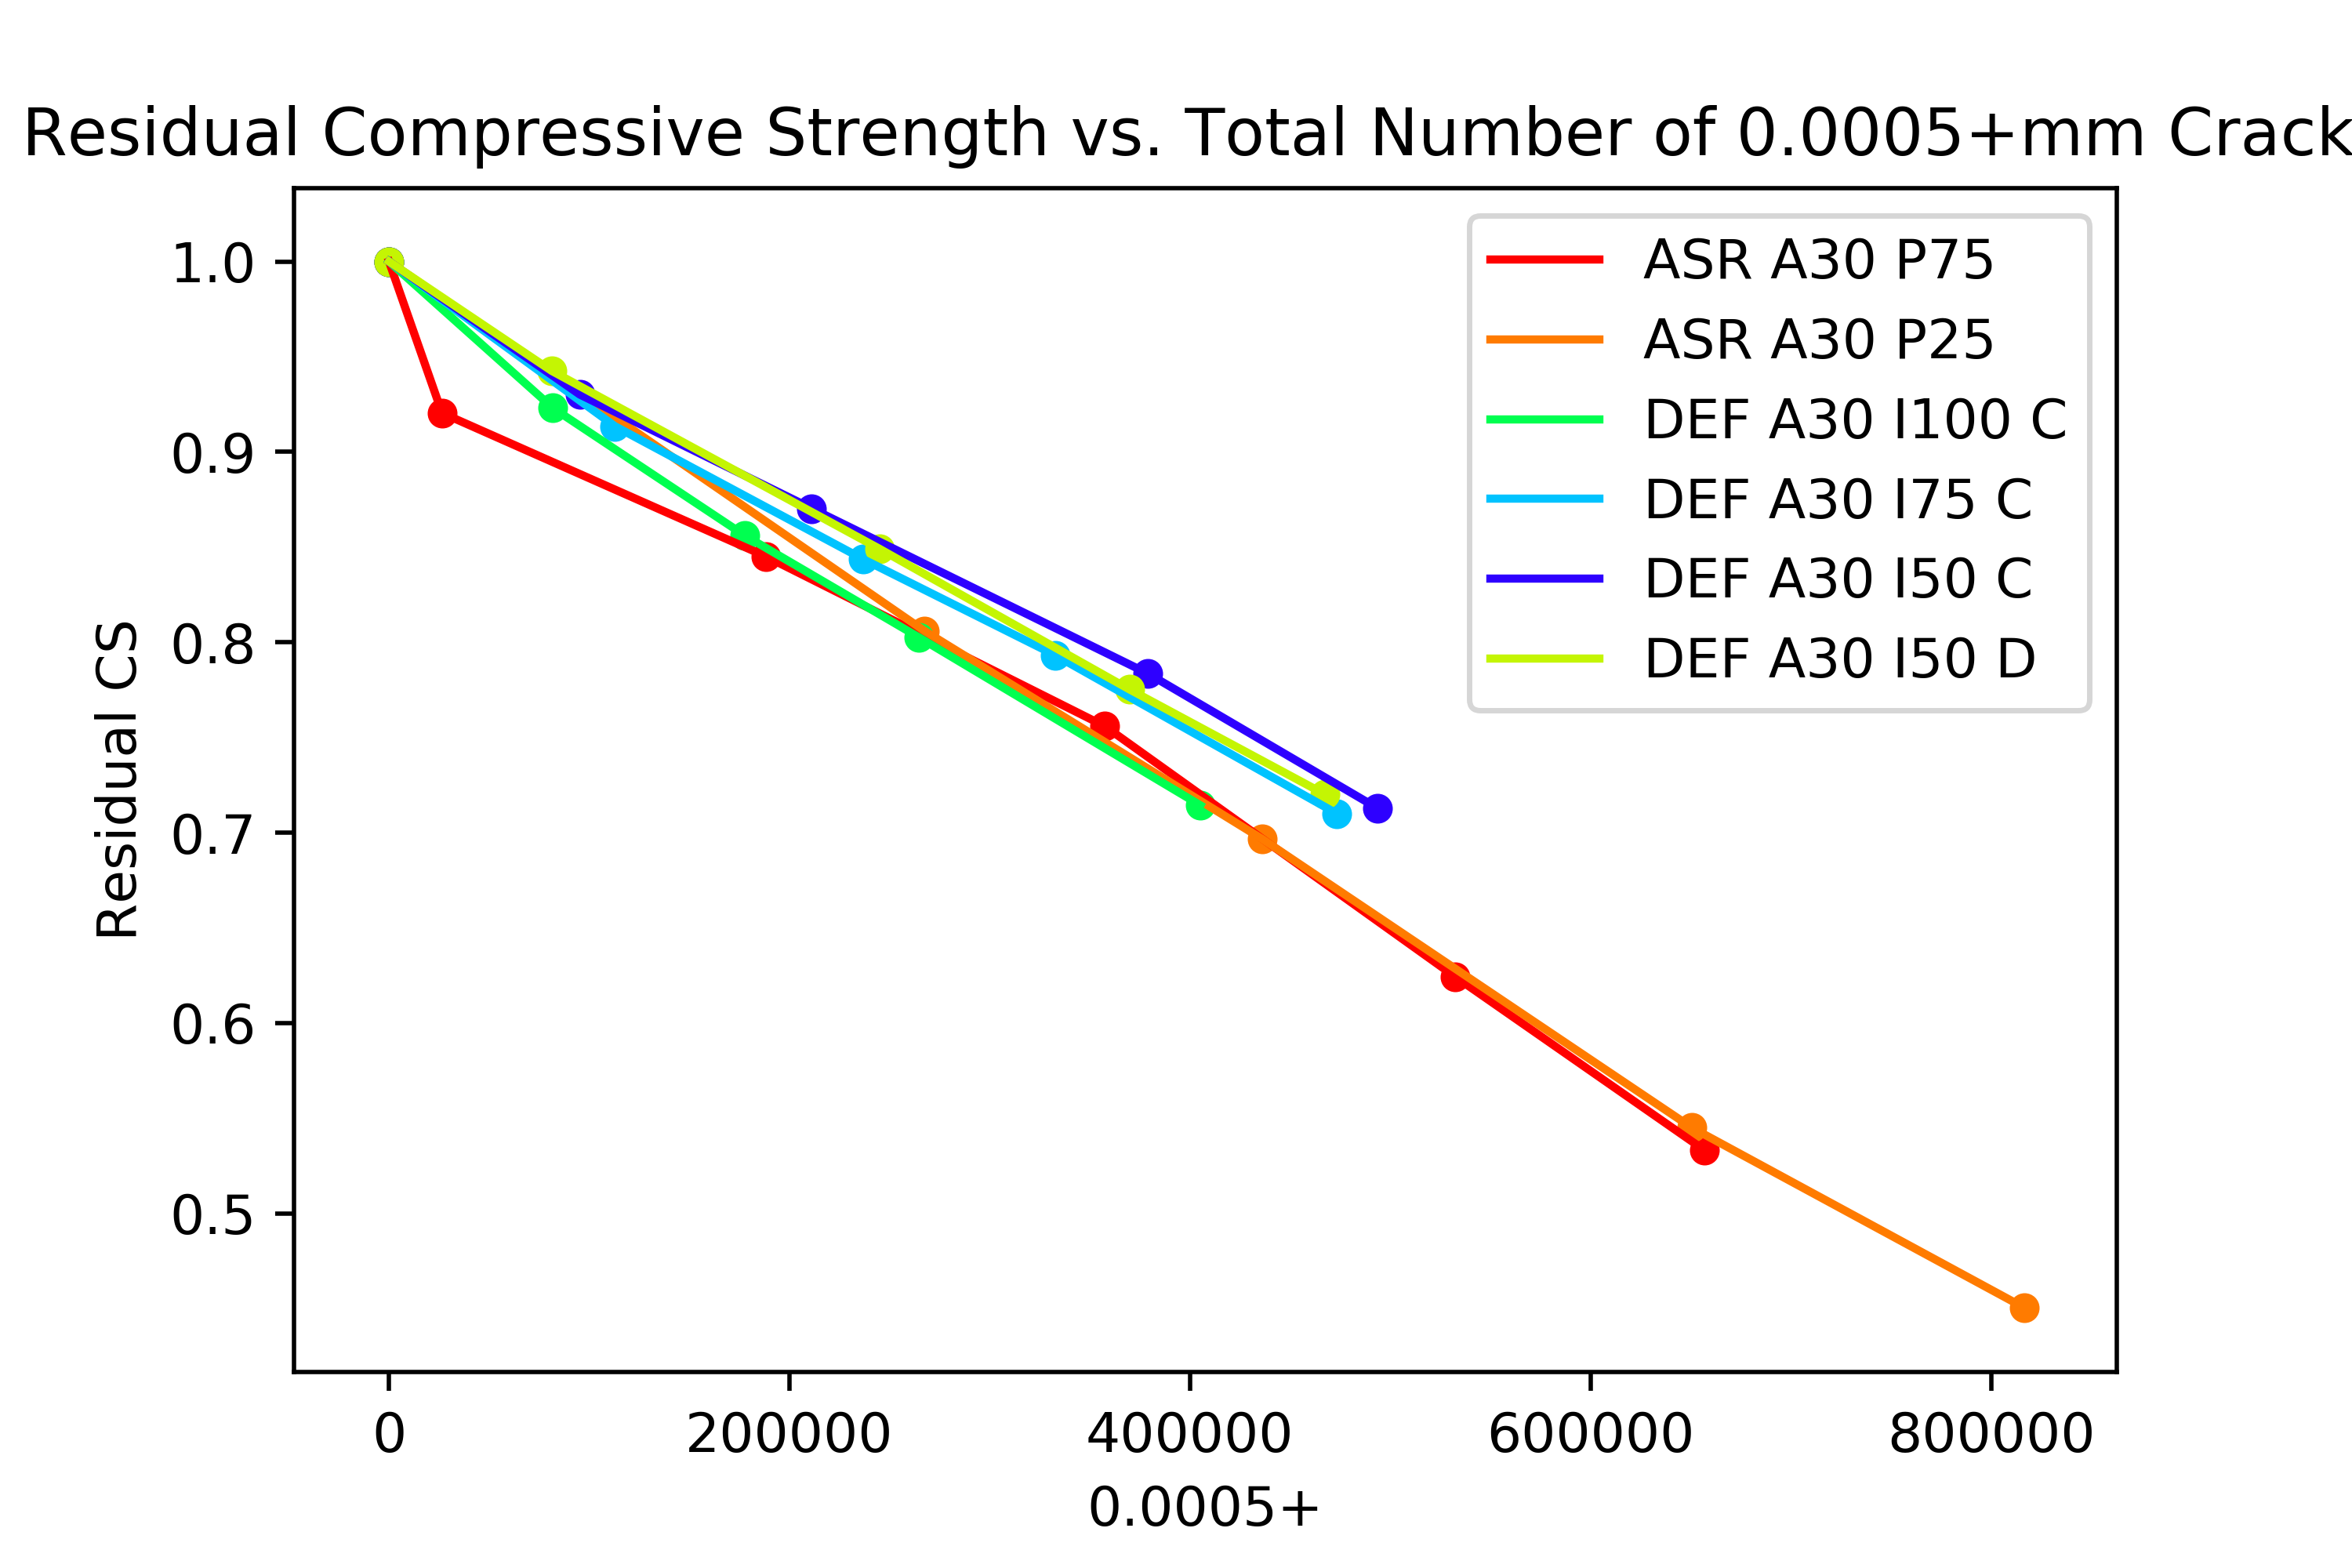
\includegraphics[width=.8\linewidth]{Files/exp_3D/Residual_Compressive_Strength_vs_Total_Number_of_0005_Cracks.png}
  \caption{Residual Compressive Strength vs. Total Number of Cracks over 0.0005mm}
  \label{fig:Total_Number_of_Cracks_0.0005+}
\end{figure}



This time clear linear relationship between the number of cracks larger than 0.0005mm and the reducing in its compressive strength can be seen here, both in ASR expansion and DEF expansion.

This result implied that while the expansion mechanism and cracking pattern can be different in ASR and DEF expansion, the residual mechanical properties, for example, the compressive strength, is determined by the existence of larger cracks (0.0005mm+ here). This may offer us a new direction in the analysis the residual capacity of the expanded concrete structure.


\begin{figure}[ht]
\centering
    %*******
    \begin{subfigure}{.33\textwidth}
      \centering
      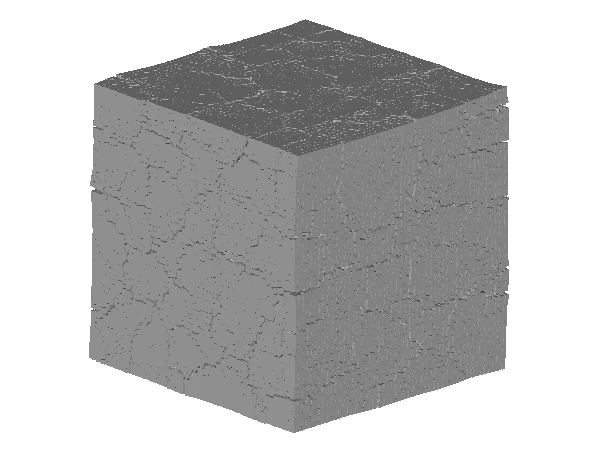
\includegraphics[width=.8\linewidth]{Files/exp_3D/ASR/A30P75_3_3d.png}
    \end{subfigure}%
    %*******
    \begin{subfigure}{.33\textwidth}
      \centering
      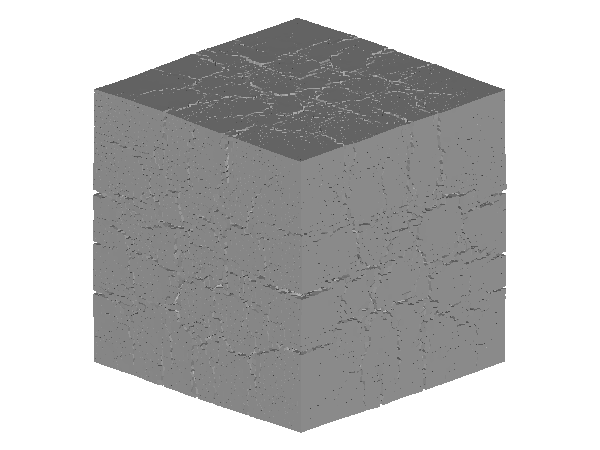
\includegraphics[width=.8\linewidth]{Files/exp_3D/DEF/A30X0C_3_3d.png}
    \end{subfigure}%
    %*******
    \begin{subfigure}{.33\textwidth}
      \centering
      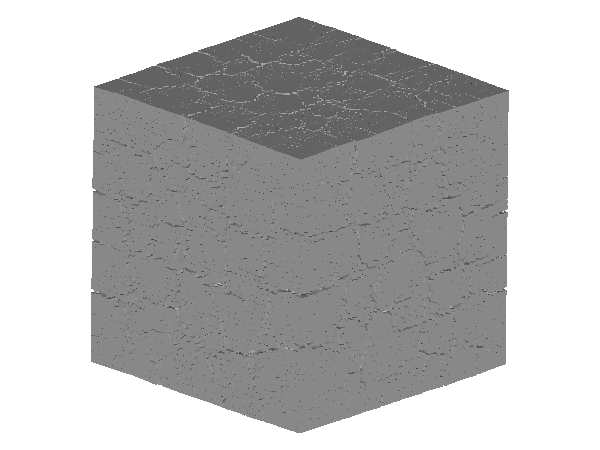
\includegraphics[width=.8\linewidth]{Files/exp_3D/DEF/A30X-5C_3_3d.png}
    \end{subfigure}
    %*******
    %*******
    \begin{subfigure}{.33\textwidth}
      \centering
      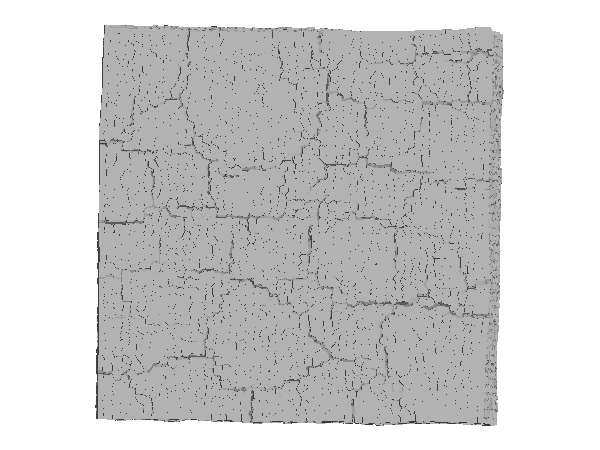
\includegraphics[width=.8\linewidth]{Files/exp_3D/ASR/A30P75_3_3ds.png}
      \caption{ASR A30 P75 Case 3 \\ Surface Crack}
    \end{subfigure}%
    %*******
    \begin{subfigure}{.33\textwidth}
      \centering
      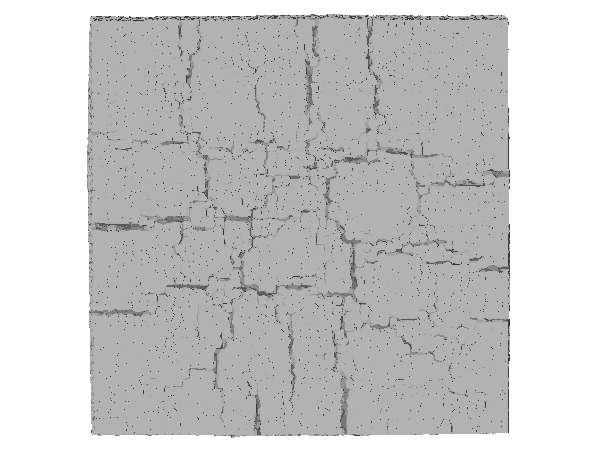
\includegraphics[width=.8\linewidth]{Files/exp_3D/DEF/A30X0C_3_3ds.png}
      \caption{DEF A30 I50 Case 3 \\ Surface Crack}
    \end{subfigure}%
    %*******
    \begin{subfigure}{.33\textwidth}
      \centering
      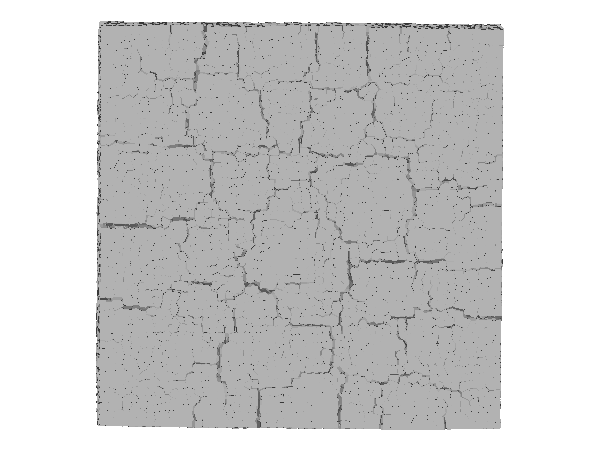
\includegraphics[width=.8\linewidth]{Files/exp_3D/DEF/A30X-5C_3_3ds.png}
      \caption{DEF A30 I75 Case 3 \\ Surface Crack}
    \end{subfigure}
    %*******
    %*******
    \begin{subfigure}{.33\textwidth}
      \centering
      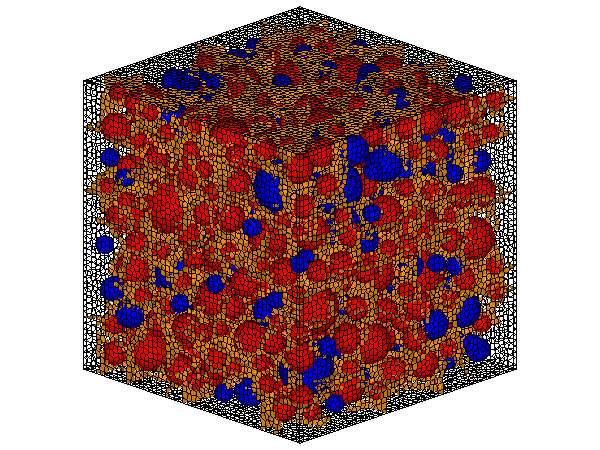
\includegraphics[width=0.8\linewidth]{Files/exp_3D/ASR/A30P75_3_c.png}
      \caption{ASR A30 P75 Case 3 \\ Internal Stress}
    \end{subfigure}%
    %*******
    \begin{subfigure}{.33\textwidth}
      \centering
      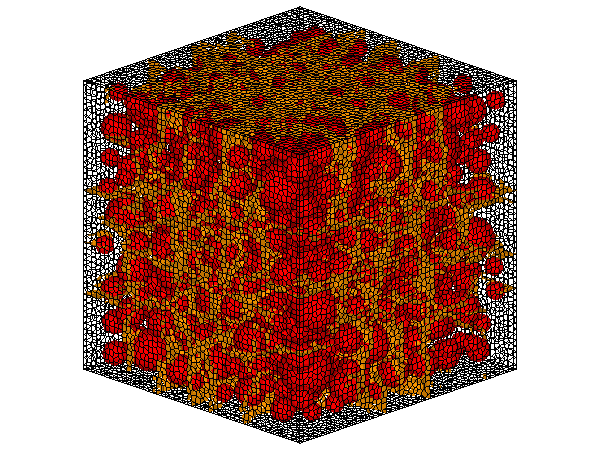
\includegraphics[width=0.8\linewidth]{Files/exp_3D/DEF/A30X0C_3_c.png}
      \caption{DEF A30 I50 Case 3 \\ Internal Stress}
    \end{subfigure}%
    %*******
    \begin{subfigure}{.33\textwidth}
      \centering
      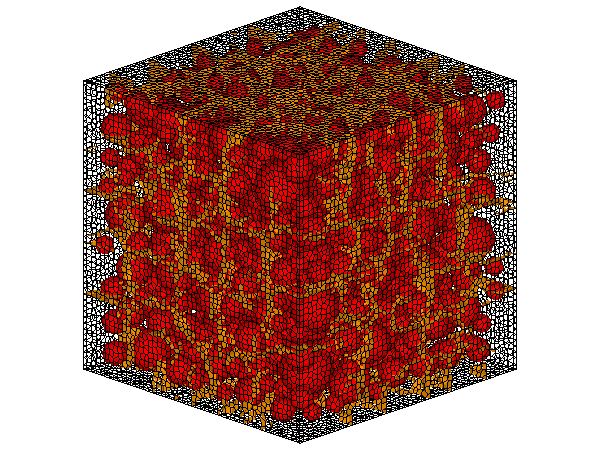
\includegraphics[width=0.8\linewidth]{Files/exp_3D/DEF/A30X-5C_3_c.png}
      \caption{DEF A30 I75 Case 3 \\ Internal Stress}
    \end{subfigure}
    %*******    
    %*******
    \begin{subfigure}{.33\textwidth}
      \centering
      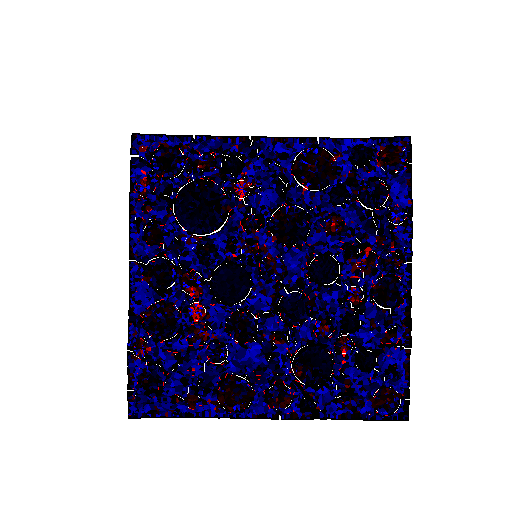
\includegraphics[width=1.0\linewidth]{Files/exp_3D/ASR/A30P75_3_stress.png}
      \caption{ASR A30 P75 Case 3 \\ Internal Stress}
    \end{subfigure}%
    %*******
    \begin{subfigure}{.33\textwidth}
      \centering
      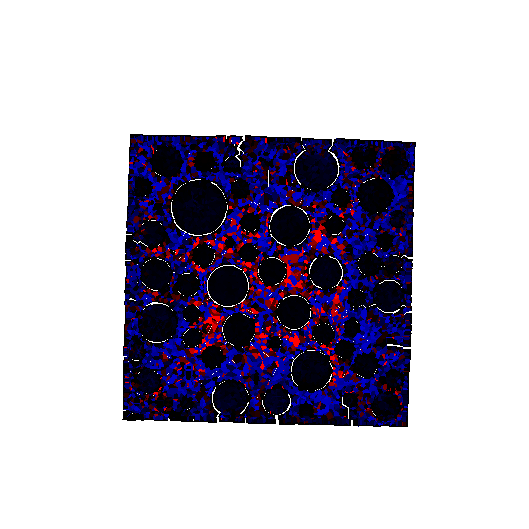
\includegraphics[width=1.0\linewidth]{Files/exp_3D/DEF/A30X0C_3_stress.png}
      \caption{DEF A30 I50 Case 3 \\ Internal Stress}
    \end{subfigure}%
    %*******
    \begin{subfigure}{.33\textwidth}
      \centering
      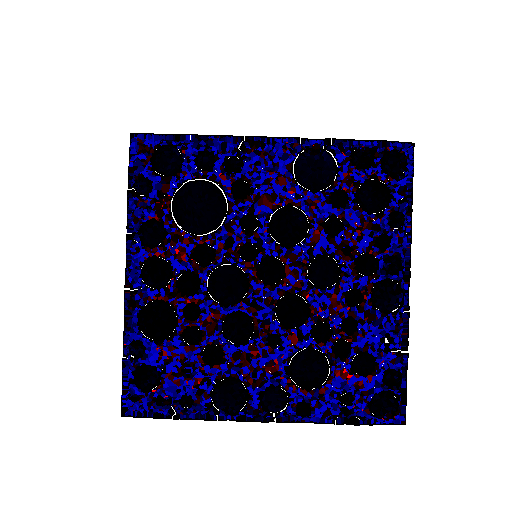
\includegraphics[width=1.0\linewidth]{Files/exp_3D/DEF/A30X-5C_3_stress.png}
      \caption{DEF A30 I75 Case 3 \\ Internal Stress}
    \end{subfigure}
    %*******
  \caption{Cracking Pattern Compare}
  \label{fig:ASR_A30P75_3_3D}
\end{figure}

\begin{table}[ht!]
\centering
\begin{tabular}{ |p{4cm}|p{2cm}|p{3cm}|p{3cm}| }
 \hline
 Case &  Final Expansion  & Number of cracked face over 0.0005mm & Residual Compressive Strength\\ [0.5ex]
 \hline
 ASR A30P75 Case 3 & 0.4223 & 357498 & 0.7559 \\ \hline
 DEF A30I50 Case 3 & 0.5795 & 379069 & 0.7835 \\ \hline
 ASR A30I75 Case 3 & 0.5118 & 332827 & 0.7931 \\
 \hline
\end{tabular}
\caption{One Dimensional Expansion Ratio in Single ASR Model Simulation}
\label{table:ASR_30_EXP}
\end{table}


\section{Residual Capabilities after Combination of ASR and DEF Expansion}

\section{Conclusion}
